\documentclass[12pt,a4paper]{report}

% 套件
\usepackage[utf8]{inputenc}
\usepackage[T1]{fontenc}
\usepackage[lining]{ebgaramond}              % EB Garamond 字體（lining numerals，數字齊線）
\usepackage[cmintegrals,cmbraces]{newtxmath} % 數學公式相容字體
\usepackage{microtype}                       % 微排版優化
\usepackage{geometry}
\usepackage{tabularx}        % 自動撐滿頁寬的表格
\usepackage{graphicx}
\usepackage{longtable}
\usepackage{booktabs}
\usepackage{array}
\usepackage{listings}
\usepackage{xcolor}
\usepackage{hyperref}
\usepackage{amsmath}
\usepackage{pdflscape}
\usepackage{float}

% 頁面設定
\geometry{
    left=1.2cm,
    right=1.2cm,
    top=2.5cm,
    bottom=2.5cm
}

% Verilog 程式碼設定
\lstdefinestyle{verilog}{
    language=Verilog,
    basicstyle=\ttfamily\footnotesize,
    keywordstyle=\color{blue}\bfseries,
    commentstyle=\color{green!60!black}\itshape,
    stringstyle=\color{red},
    numbers=left,
    numberstyle=\tiny\color{gray},
    stepnumber=1,
    numbersep=8pt,
    backgroundcolor=\color{gray!10},
    frame=single,
    breaklines=true,
    breakatwhitespace=false,
    tabsize=4,
    captionpos=b
}

\lstset{style=verilog}

% 顏色定義（對標樣本深紅色主題）
\definecolor{crimson}{RGB}{153, 0, 0}
\definecolor{coffee}{RGB}{101, 67, 33}

% 超連結設定
\hypersetup{
    colorlinks=true,
    linkcolor=crimson,
    urlcolor=crimson,
    citecolor=crimson
}

% 章節標題樣式（對標樣本右對齊大號 serif）
\usepackage{titlesec}
\titleformat{\chapter}[display]
  {\normalfont\huge\bfseries\raggedleft}
  {\chaptertitlename\ \thechapter}
  {0pt}{}[\vspace{0.5em}]
\titleformat{\section}{\normalfont\Large\bfseries}{\thesection}{1em}{}
\titleformat{\subsection}{\normalfont\large\bfseries}{\thesubsection}{1em}{}

\begin{document}

\pagestyle{plain}

% longtable 水平置中
\setlength\LTleft{0pt plus 1fill}
\setlength\LTright{0pt plus 1fill}

% 自訂封面
\begin{titlepage}
\centering
\vspace*{3cm}

{\fontsize{28}{34}\selectfont\bfseries 32-bit RISC-V Processor\par}
\vspace{0.6em}
{\fontsize{16}{20}\selectfont\bfseries Design Specification\par}

\vspace{1.5cm}
\textcolor{coffee}{\rule{0.6\linewidth}{1.2pt}}
\vspace{1.5cm}

{\large\bfseries Author}\par
\vspace{0.4em}
{\large \href{https://github.com/akira2963753}{Marco}}\par

\vspace{2cm}

{\large\bfseries Development Environment}\par
\vspace{0.8em}
\begin{tabular}{rl}
    \textbf{HDL}     & Verilog HDL \\[4pt]
    \textbf{EDA Tool}  & Vivado 2025.1 \\[4pt]
    \textbf{ISA}       & RV32I + RV32M \\[4pt]
    \textbf{Target}    & Xilinx ZCU104 \\
\end{tabular}

\vfill

\textcolor{coffee}{\rule{0.6\linewidth}{0.6pt}}\par
\vspace{0.5em}
{\small Version 1.0 \quad\textbullet\quad February 2026}

\end{titlepage}

\tableofcontents
\newpage

\chapter{Abstract \& Introduction}

This project is based on \href{https://github.com/akira2963753/Pipelined-RV32-SoC/tree/main?tab=readme-ov-file}{Computer Organization Course} and \href{https://cs61c.org/}{UC Berkeley CS 61C.} The goal was to design a 32-bit pipelined RISC-V CPU supporting RV32I and RV32M, including Forwarding, Hazard Detection, Flush Detection, Dynamic Branch Prediction, and two Caches with AXI4-Lite Bus to BRAM. The final design was implemented and verified on FPGA.

Our development process follows a modular approach, beginning with the core execution unit and progressively expanding into a complete system-on-chip (SoC) architecture. The project is structured into four sequential phases :

\begin{enumerate}
    \item \textbf{Core Processor Design:} Implement a 5-stage pipelined RISC-V CPU supporting both the RV32I (Base Integer) and RV32M (Integer Multiplication and Division) instruction sets, including Forwarding, Hazard Detection, Flush Detection, and Dynamic Branch Prediction.

    \item \textbf{Bus Infrastructure:} Design an AXI4-Lite bus interface compliant with the ARM AXI protocol, followed by comprehensive system-level testing by interfacing the bus with BRAM (Block RAM).

    \item \textbf{Memory Hierarchy:} Develop independent Instruction and Data Caches, and integrate them with the AXI4-Lite Bus and BRAM to verify cache coherency and proper timing behaviour.

    \item \textbf{Full System Integration:} Integrate both caches into the pipelined RISC-V CPU, forming a complete processor connected to BRAM via the AXI4-Lite interconnect, and deploy the final design onto an FPGA.
\end{enumerate}

\medskip
\noindent The complete source code, RTL design files, testbenches, and verification scripts for this project are publicly available on GitHub:

\medskip
\noindent\href{https://github.com/akira2963753/Pipelined-RV32-SoC}{\texttt{https://github.com/akira2963753/Pipelined-RV32-SoC}}


\chapter{RV32I \& RV32M}
\newpage
\section{The RV32I \& RV32M Instruction Table supported by this processor}

\begin{longtable}{|l|p{6cm}|c|c|c|c|c|c|}
\caption{R-Type Instructions} \\
\hline
\textbf{R-Type} & \textbf{Description} & \textbf{Funct7} & \textbf{Rs2} & \textbf{Rs1} & \textbf{Funct3} & \textbf{Rd} & \textbf{Opcode} \\
\hline
\endfirsthead

\multicolumn{8}{c}{\tablename\ \thetable\ -- \textit{Continued from previous page}} \\
\hline
\textbf{R-Type} & \textbf{Description} & \textbf{Funct7} & \textbf{Rs2} & \textbf{Rs1} & \textbf{Funct3} & \textbf{Rd} & \textbf{Opcode} \\
\hline
\endhead

\hline
\multicolumn{8}{r}{\textit{Continued on next page}} \\
\endfoot

\hline
\endlastfoot

ADD & Rd = Rs1 + Rs2 & 0000000 & Rs2 & Rs1 & 000 & Rd & 0110011 \\
\hline
SUB & Rd = Rs1 - Rs2 & 0100000 & Rs2 & Rs1 & 000 & Rd & 0110011 \\
\hline
SLL & Rd = Rs1 $<<$ Rs2 & 0000000 & Rs2 & Rs1 & 001 & Rd & 0110011 \\
\hline
SLT & Rd = (Rs1 $<$ Rs2) & 0000000 & Rs2 & Rs1 & 010 & Rd & 0110011 \\
\hline
SLTU & Rd = (Rs1 $<$ Rs2) & 0000000 & Rs2 & Rs1 & 011 & Rd & 0110011 \\
\hline
XOR & Rd = Rs1 $\oplus$ Rs2 & 0000000 & Rs2 & Rs1 & 100 & Rd & 0110011 \\
\hline
SRL & Rd = Rs1 $>>$ Rs2 & 0000000 & Rs2 & Rs1 & 101 & Rd & 0110011 \\
\hline
SRA & Rd = Rs1 $>>>$ Rs2 & 0100000 & Rs2 & Rs1 & 101 & Rd & 0110011 \\
\hline
OR & Rd = Rs1 $|$ Rs2 & 0000000 & Rs2 & Rs1 & 110 & Rd & 0110011 \\
\hline
AND & Rd = Rs1 $\&$ Rs2 & 0000000 & Rs2 & Rs1 & 111 & Rd & 0110011 \\
\hline
MUL & Rd = (Rs1 $\times$ Rs2)[31:0] & 0000001 & Rs2 & Rs1 & 000 & Rd & 0110011 \\
\hline
MULH & Rd = (Rs1 $\times$ Rs2)[63:32] & 0000001 & Rs2 & Rs1 & 001 & Rd & 0110011 \\
\hline
MULHSU & Rd = (Rs1 $\times$ Rs2[U])[63:32] & 0000001 & Rs2 & Rs1 & 010 & Rd & 0110011 \\
\hline
MULHU & Rd = (Rs1[U] $\times$ Rs2[U])[63:32] & 0000001 & Rs2 & Rs1 & 011 & Rd & 0110011 \\
\hline
DIV & Rd = Rs1 / Rs2 & 0000001 & Rs2 & Rs1 & 100 & Rd & 0110011 \\
\hline
DIVU & Rd = Rs1[U] / Rs2[U] & 0000001 & Rs2 & Rs1 & 101 & Rd & 0110011 \\
\hline
REM & Rd = Rs1 \% Rs2 & 0000001 & Rs2 & Rs1 & 110 & Rd & 0110011 \\
\hline
REMU & Rd = Rs1[U] \% Rs2[U] & 0000001 & Rs2 & Rs1 & 111 & Rd & 0110011 \\
\hline
\end{longtable}

\begin{longtable}{|l|p{6cm}|c|c|c|c|c|c|}
\caption{I-Type Instructions} \\
\hline
\textbf{I-Type} & \textbf{Description} & \textbf{Imm[11:0]} & \textbf{-} & \textbf{Rs1} & \textbf{Funct3} & \textbf{Rd} & \textbf{Opcode} \\
\hline
\endfirsthead

\multicolumn{8}{c}{\tablename\ \thetable\ -- \textit{Continued from previous page}} \\
\hline
\textbf{I-Type} & \textbf{Description} & \textbf{Imm[11:0]} & \textbf{-} & \textbf{Rs1} & \textbf{Funct3} & \textbf{Rd} & \textbf{Opcode} \\
\hline
\endhead

\hline
\multicolumn{8}{r}{\textit{Continued on next page}} \\
\endfoot

\hline
\endlastfoot

ADDI & Rd = Rs1 + Imm & Imm[11:0] & - & Rs1 & 000 & Rd & 0010011 \\
\hline
SUBI & Rd = Rs1 - Imm & Imm[11:0] & - & Rs1 & 001 & Rd & 0010011 \\
\hline
SLTI & Rd = (Rs1 $<$ Imm) & Imm[11:0] & - & Rs1 & 010 & Rd & 0010011 \\
\hline
SLTIU & Rd = (Rs1 $<$ Imm) & Imm[11:0] & - & Rs1 & 011 & Rd & 0010011 \\
\hline
XORI & Rd = Rs1 $\oplus$ Imm & Imm[11:0] & - & Rs1 & 100 & Rd & 0010011 \\
\hline
ORI & Rd = Rs1 $|$ Imm & Imm[11:0] & - & Rs1 & 110 & Rd & 0010011 \\
\hline
ANDI & Rd = Rs1 $\&$ Imm & Imm[11:0] & - & Rs1 & 111 & Rd & 0010011 \\
\hline
JALR & Rd = PC + 4, PC = Rs1 + Imm $\&$ (-1) & Imm[11:0] & - & Rs1 & 000 & Rd & 1100111 \\
\hline
SLLI & Rd = Rs1 $<<$ shamt & 0000000 & Shamt & Rs1 & 001 & Rd & 0010011 \\
\hline
SRLI & Rd = Rs1 $>>$ shamt & 0000000 & Shamt & Rs1 & 101 & Rd & 0010011 \\
\hline
SRAI & Rd = Rs1 $>>>$ shamt & 0100000 & Shamt & Rs1 & 101 & Rd & 0010011 \\
\hline
LB & Rd[7:0] = M[Rs1+Imm] & Imm[11:0] & - & Rs1 & 000 & Rd & 0000011 \\
\hline
LH & Rd[15:0] = M[Rs1+Imm] & Imm[11:0] & - & Rs1 & 001 & Rd & 0000011 \\
\hline
LW & Rd = M[Rs1+Imm] & Imm[11:0] & - & Rs1 & 010 & Rd & 0000011 \\
\hline
LBU & Rd[7:0] = M[Rs1+Imm] & Imm[11:0] & - & Rs1 & 011 & Rd & 0000011 \\
\hline
LHU & Rd[15:0] = M[Rs1+Imm] & Imm[11:0] & - & Rs1 & 100 & Rd & 0000011 \\
\hline
CSRRW & Rd = CSR[csr]; CSR[csr] = Rs1 & CSR[11:0] & - & Rs1 & 001 & Rd & 1110011 \\
\hline
CSRRS & Rd = CSR[csr]; CSR[csr] $|=$ Rs1 & CSR[11:0] & - & Rs1 & 010 & Rd & 1110011 \\
\hline
CSRRC & Rd = CSR[csr]; CSR[csr] \&= $\sim$Rs1 & CSR[11:0] & - & Rs1 & 011 & Rd & 1110011 \\
\hline
\end{longtable}

\begin{longtable}{|l|p{6cm}|c|c|c|c|c|c|}
\caption{S-Type Instructions} \\
\hline
\textbf{S-Type} & \textbf{Description} & \textbf{Imm[11:5]} & \textbf{Rs2} & \textbf{Rs1} & \textbf{Funct3} & \textbf{Imm[4:0]} & \textbf{Opcode} \\
\hline
\endfirsthead
\hline
\endlastfoot

SB & M[Rs1 + Imm][7:0] = Rs2[7:0] & Imm[11:5] & Rs2 & Rs1 & 000 & Imm[4:0] & 0100011 \\
\hline
SH & M[Rs1 + Imm][15:0] = Rs2[15:0] & Imm[11:5] & Rs2 & Rs1 & 001 & Imm[4:0] & 0100011 \\
\hline
SW & M[Rs1 + Imm] = Rs2 & Imm[11:5] & Rs2 & Rs1 & 010 & Imm[4:0] & 0100011 \\
\hline
\end{longtable}

\vspace{1.5em}

\begin{longtable}{|l|p{5cm}|c|c|c|c|c|c|}
\caption{B-Type Instructions} \\
\hline
\textbf{B-Type} & \textbf{Description} & \textbf{Imm[12|10:5]} & \textbf{Rs2} & \textbf{Rs1} & \textbf{Funct3} & \textbf{Imm[4:1|11]} & \textbf{Opcode} \\
\hline
\endfirsthead
\hline
\endlastfoot

BEQ & if (Rs1 == Rs2) PC = PC + Imm & Imm[12|10:5] & Rs2 & Rs1 & 000 & Imm[4:1|11] & 1100011 \\
\hline
BNE & if (Rs1 != Rs2) PC = PC + Imm & Imm[12|10:5] & Rs2 & Rs1 & 001 & Imm[4:1|11] & 1100011 \\
\hline
BLT & if (Rs1 $<$ Rs2) PC = PC + Imm & Imm[12|10:5] & Rs2 & Rs1 & 100 & Imm[4:1|11] & 1100011 \\
\hline
BGE & if (Rs1 $\geq$ Rs2) PC = PC + Imm & Imm[12|10:5] & Rs2 & Rs1 & 101 & Imm[4:1|11] & 1100011 \\
\hline
BLTU & if (Rs1[U] $<$ Rs2[U]) PC = PC + Imm & Imm[12|10:5] & Rs2 & Rs1 & 110 & Imm[4:1|11] & 1100011 \\
\hline
BGEU & if (Rs1[U] $\geq$ Rs2[U]) PC = PC + Imm & Imm[12|10:5] & Rs2 & Rs1 & 111 & Imm[4:1|11] & 1100011 \\
\hline
\end{longtable}

\vspace{1.5em}

\begin{longtable}{|l|p{6cm}|c|c|c|c|c|c|}
\caption{U-Type Instructions} \\
\hline
\textbf{U-Type} & \textbf{Description} & \multicolumn{4}{c|}{\textbf{Imm[31:12]}} & \textbf{Rd} & \textbf{Opcode} \\
\hline
\endfirsthead
\hline
\endlastfoot

LUI & Rd = Imm $<<$ 12 & \multicolumn{4}{c|}{Imm[31:12]} & Rd & 0110111 \\
\hline
AUIPC & Rd = PC + (Imm $<<$ 12) & \multicolumn{4}{c|}{Imm[31:12]} & Rd & 0010111 \\
\hline
\end{longtable}

\vspace{1.5em}

\begin{longtable}{|l|p{6cm}|c|c|c|c|c|c|}
\caption{J-Type Instructions} \\
\hline
\textbf{J-Type} & \textbf{Description} & \textbf{Imm[20|10:1|11|19:12]} & \textbf{-} & \textbf{-} & \textbf{-} & \textbf{Rd} & \textbf{Opcode} \\
\hline
\endfirsthead
\hline
\endlastfoot

JAL & Rd = PC + 4, PC = PC + Imm & Imm[20|10:1|11|19:12] & - & - & - & Rd & 1101111 \\
\hline
\end{longtable}

\chapter{RISC-V Core}
\newpage
\section{Processor Core}

\begin{figure}[htbp]
    \centering
    \includegraphics[width=\textwidth]{RISC-V Processor.png}
    \caption{RISC-V Core System Framework Diagram Supporting RV32I and RV32M}
    \label{fig:processor_core}
\end{figure}

\subsection{Datapath Descriptions for All Instructions}

Due to the large size of the datapath table, it will be presented across multiple pages.

\begin{longtable}{|l|p{12cm}|}
\caption{Instruction Operation Datapath Description} \\
\hline
\textbf{Instruction} & \textbf{Operation Datapath Description} \\
\hline
\endfirsthead

\multicolumn{2}{c}{\tablename\ \thetable\ -- \textit{Continued from previous page}} \\
\hline
\textbf{Instruction} & \textbf{Operation Datapath Description} \\
\hline
\endhead

\hline
\multicolumn{2}{r}{\textit{Continued on next page}} \\
\endfoot

\hline
\endlastfoot

ADD Rd, Rs1, Rs2 & After decoding in the ID stage, Forwarding A \& B = 0, selecting EX\_Rd\_Data as the data for Rs1 and Rs2. EX\_ALU\_src1 and EX\_ALU\_src2 = 0, allowing the ALU to successfully add the two data values. Then in the WB stage, with WB\_WB\_sel = 0, WB\_ALU\_Result is written back. \\
\hline

SUB Rd, Rs1, Rs2 & After decoding in the ID stage, Forwarding A \& B = 0, selecting EX\_Rd\_Data as the data for Rs1 and Rs2. EX\_ALU\_src1 and EX\_ALU\_src2 = 0, allowing the ALU to successfully subtract the two data values. Then in the WB stage, with WB\_WB\_sel = 0, WB\_ALU\_Result is written back. \\
\hline

SLL Rd, Rs1, Rs2 & After decoding in the ID stage, Forwarding A \& B = 0, selecting EX\_Rd\_Data as the data for Rs1 and Rs2. EX\_ALU\_src1 and EX\_ALU\_src2 = 0, allowing the ALU to successfully perform Rs1 $<<$ Rs2. Then in the WB stage, with WB\_WB\_sel = 0, WB\_ALU\_Result is written back. \\
\hline

SLT Rd, Rs1, Rs2 & After decoding in the ID stage, Forwarding A \& B = 0, selecting EX\_Rd\_Data as the data for Rs1 and Rs2. EX\_ALU\_src1 and EX\_ALU\_src2 = 0, allowing the ALU to determine whether Rs1 is less than Rs2. Then in the WB stage, with WB\_WB\_sel = 0, WB\_ALU\_Result is written back. \\
\hline

SLTU Rd, Rs1, Rs2 & After decoding in the ID stage, Forwarding A \& B = 0, selecting EX\_Rd\_Data as the data for Rs1 and Rs2. EX\_ALU\_src1 and EX\_ALU\_src2 = 0, allowing the ALU to determine whether Rs1 [U] is less than Rs2 [U]. Then in the WB stage, with WB\_WB\_sel = 0, WB\_ALU\_Result is written back. \\
\hline

XOR Rd, Rs1, Rs2 & After decoding in the ID stage, Forwarding A \& B = 0, selecting EX\_Rd\_Data as the data for Rs1 and Rs2. EX\_ALU\_src1 and EX\_ALU\_src2 = 0, allowing the ALU to successfully perform Rs1 $\oplus$ Rs2. Then in the WB stage, with WB\_WB\_sel = 0, WB\_ALU\_Result is written back. \\
\hline

SRL Rd, Rs1, Rs2 & After decoding in the ID stage, Forwarding A \& B = 0, selecting EX\_Rd\_Data as the data for Rs1 and Rs2. EX\_ALU\_src1 and EX\_ALU\_src2 = 0, allowing the ALU to successfully perform Rs1 $>>$ Rs2. Then in the WB stage, with WB\_WB\_sel = 0, WB\_ALU\_Result is written back. \\
\hline

SRA Rd, Rs1, Rs2 & After decoding in the ID stage, Forwarding A \& B = 0, selecting EX\_Rd\_Data as the data for Rs1 and Rs2. EX\_ALU\_src1 and EX\_ALU\_src2 = 0, allowing the ALU to successfully perform Rs1 $>>>$ Rs2. Then in the WB stage, with WB\_WB\_sel = 0, WB\_ALU\_Result is written back. \\
\hline

OR Rd, Rs1, Rs2 & After decoding in the ID stage, Forwarding A \& B = 0, selecting EX\_Rd\_Data as the data for Rs1 and Rs2. EX\_ALU\_src1 and EX\_ALU\_src2 = 0, allowing the ALU to successfully perform Rs1 $|$ Rs2. Then in the WB stage, with WB\_WB\_sel = 0, WB\_ALU\_Result is written back. \\
\hline

AND Rd, Rs1, Rs2 & After decoding in the ID stage, Forwarding A \& B = 0, selecting EX\_Rd\_Data as the data for Rs1 and Rs2. EX\_ALU\_src1 and EX\_ALU\_src2 = 0, allowing the ALU to successfully perform Rs1 $\&$ Rs2. Then in the WB stage, with WB\_WB\_sel = 0, WB\_ALU\_Result is written back. \\
\hline

MUL Rd, Rs1, Rs2 & After decoding in the ID stage, Forwarding A \& B = 0, selecting EX\_Rd\_Data as the data for Rs1 and Rs2. EX\_ALU\_src1 and EX\_ALU\_src2 = 0, allowing the ALU to successfully perform Rs1 $\times$ Rs2 and output the lower 32 bits. Then in the WB stage, with WB\_WB\_sel = 0, WB\_ALU\_Result is written back. \\
\hline

MULH Rd, Rs1, Rs2 & After decoding in the ID stage, Forwarding A \& B = 0, selecting EX\_Rd\_Data as the data for Rs1 and Rs2. EX\_ALU\_src1 and EX\_ALU\_src2 = 0, allowing the ALU to successfully perform Rs1 $\times$ Rs2 and output the upper 32 bits. Then in the WB stage, with WB\_WB\_sel = 0, WB\_ALU\_Result is written back. \\
\hline

MULHSU Rd, Rs1, Rs2 & After decoding in the ID stage, Forwarding A \& B = 0, selecting EX\_Rd\_Data as the data for Rs1 and Rs2. EX\_ALU\_src1 and EX\_ALU\_src2 = 0, allowing the ALU to successfully perform Rs1 $\times$ Rs2 [U] and output the upper 32 bits. Then in the WB stage, with WB\_WB\_sel = 0, WB\_ALU\_Result is written back. \\
\hline

MULHU Rd, Rs1, Rs2 & After decoding in the ID stage, Forwarding A \& B = 0, selecting EX\_Rd\_Data as the data for Rs1 and Rs2. EX\_ALU\_src1 and EX\_ALU\_src2 = 0, allowing the ALU to successfully perform Rs1 [U] $\times$ Rs2 [U] and output the upper 32 bits. Then in the WB stage, with WB\_WB\_sel = 0, WB\_ALU\_Result is written back. \\
\hline

DIV Rd, Rs1, Rs2 & After decoding in the ID stage, Forwarding A \& B = 0, selecting EX\_Rd\_Data as the data for Rs1 and Rs2. EX\_ALU\_src1 and EX\_ALU\_src2 = 0, allowing the ALU to successfully perform Rs1 / Rs2. Then in the WB stage, with WB\_WB\_sel = 0, WB\_ALU\_Result is written back. \\
\hline

DIVU Rd, Rs1, Rs2 & After decoding in the ID stage, Forwarding A \& B = 0, selecting EX\_Rd\_Data as the data for Rs1 and Rs2. EX\_ALU\_src1 and EX\_ALU\_src2 = 0, allowing the ALU to successfully perform Rs1 [U] / Rs2 [U]. Then in the WB stage, with WB\_WB\_sel = 0, WB\_ALU\_Result is written back. \\
\hline

REM Rd, Rs1, Rs2 & After decoding in the ID stage, Forwarding A \& B = 0, selecting EX\_Rd\_Data as the data for Rs1 and Rs2. EX\_ALU\_src1 and EX\_ALU\_src2 = 0, allowing the ALU to successfully perform Rs1 \% Rs2. Then in the WB stage, with WB\_WB\_sel = 0, WB\_ALU\_Result is written back. \\
\hline

REMU Rd, Rs1, Rs2 & After decoding in the ID stage, Forwarding A \& B = 0, selecting EX\_Rd\_Data as the data for Rs1 and Rs2. EX\_ALU\_src1 and EX\_ALU\_src2 = 0, allowing the ALU to successfully perform Rs1 [U] \% Rs2 [U]. Then in the WB stage, with WB\_WB\_sel = 0, WB\_ALU\_Result is written back. \\
\hline

ADDI Rd, Rs1, Imm & After decoding in the ID stage, Forwarding A \& B = 0, selecting EX\_Rd\_Data as the data for Rs1 and Rs2. EX\_ALU\_src1 = 0, EX\_ALU\_src2 = 1, allowing the ALU to successfully perform Rs1 + Imm. Then in the WB stage, with WB\_WB\_sel = 0, WB\_ALU\_Result is written back. \\
\hline

SUBI Rd, Rs1, Imm & After decoding in the ID stage, Forwarding A \& B = 0, selecting EX\_Rd\_Data as the data for Rs1 and Rs2. EX\_ALU\_src1 = 0, EX\_ALU\_src2 = 1, allowing the ALU to successfully perform Rs1 - Imm. Then in the WB stage, with WB\_WB\_sel = 0, WB\_ALU\_Result is written back. \\
\hline

SLTI Rd, Rs1, Imm & After decoding in the ID stage, Forwarding A \& B = 0, selecting EX\_Rd\_Data as the data for Rs1 and Rs2. EX\_ALU\_src1 = 0, EX\_ALU\_src2 = 1, allowing the ALU to determine whether Rs1 is less than Imm. Then in the WB stage, with WB\_WB\_sel = 0, WB\_ALU\_Result is written back. \\
\hline

SLTIU Rd, Rs1, Imm & After decoding in the ID stage, Forwarding A \& B = 0, selecting EX\_Rd\_Data as the data for Rs1 and Rs2. EX\_ALU\_src1 = 0, EX\_ALU\_src2 = 1, allowing the ALU to determine whether Rs1 [U] is less than Imm [U] (though Imm is still sign-extended first). Then in the WB stage, with WB\_WB\_sel = 0, WB\_ALU\_Result is written back. \\
\hline

XORI Rd, Rs1, Imm & After decoding in the ID stage, Forwarding A \& B = 0, selecting EX\_Rd\_Data as the data for Rs1 and Rs2. EX\_ALU\_src1 = 0, EX\_ALU\_src2 = 1, allowing the ALU to successfully perform Rs1 $\oplus$ Imm. Then in the WB stage, with WB\_WB\_sel = 0, WB\_ALU\_Result is written back. \\
\hline

ORI Rd, Rs1, Imm & After decoding in the ID stage, Forwarding A \& B = 0, selecting EX\_Rd\_Data as the data for Rs1 and Rs2. EX\_ALU\_src1 = 0, EX\_ALU\_src2 = 1, allowing the ALU to successfully perform Rs1 $|$ Imm. Then in the WB stage, with WB\_WB\_sel = 0, WB\_ALU\_Result is written back. \\
\hline

ANDI Rd, Rs1, Imm & After decoding in the ID stage, Forwarding A \& B = 0, selecting EX\_Rd\_Data as the data for Rs1 and Rs2. EX\_ALU\_src1 = 0, EX\_ALU\_src2 = 1, allowing the ALU to successfully perform Rs1 $\&$ Imm. Then in the WB stage, with WB\_WB\_sel = 0, WB\_ALU\_Result is written back. \\
\hline

JALR Rd, Rs1, Imm & After decoding in the ID stage, Forwarding A \& B = 0, selecting EX\_Rd\_Data as the data for Rs1 and Rs2. EX\_ALU\_src1 = 0, EX\_ALU\_src2 = 1, allowing the ALU to successfully perform Rs1 + Imm $\&$ (-1). Then, with EX\_Jump = 1, PC\_sel = 3, setting PC = EX\_ALU\_Result. In the WB stage, WB\_WB\_sel = 1, resulting in Rd = PC + 4. \\
\hline

SLLI Rd, Rs1, Imm & After decoding in the ID stage, Forwarding A \& B = 0, selecting EX\_Rd\_Data as the data for Rs1 and Rs2. EX\_ALU\_src1 = 0, EX\_ALU\_src2 = 1, allowing the ALU to successfully perform Rs1 $<<$ Imm. Then in the WB stage, with WB\_WB\_sel = 0, WB\_ALU\_Result is written back. \\
\hline

SRLI Rd, Rs1, Imm & After decoding in the ID stage, Forwarding A \& B = 0, selecting EX\_Rd\_Data as the data for Rs1 and Rs2. EX\_ALU\_src1 = 0, EX\_ALU\_src2 = 1, allowing the ALU to successfully perform Rs1 $>>$ Imm. Then in the WB stage, with WB\_WB\_sel = 0, WB\_ALU\_Result is written back. \\
\hline

SRAI Rd, Rs1, Imm & After decoding in the ID stage, Forwarding A \& B = 0, selecting EX\_Rd\_Data as the data for Rs1 and Rs2. EX\_ALU\_src1 = 0, EX\_ALU\_src2 = 1, allowing the ALU to successfully perform Rs1 $>>>$ Imm. Then in the WB stage, with WB\_WB\_sel = 0, WB\_ALU\_Result is written back. \\
\hline

SB Rs1, Rs2, Imm & After decoding in the ID stage, Forwarding A \& B = 0, selecting EX\_Rd\_Data as the data for Rs1 and Rs2. EX\_ALU\_src1 = 0, EX\_ALU\_src2 = 1, allowing the ALU to successfully perform Rs1 + Imm to calculate the memory write address. Then, W\_STRB controls the byte write operation, writing Rs2[7:0]. \\
\hline

SH Rs1, Rs2, Imm & After decoding in the ID stage, Forwarding A \& B = 0, selecting EX\_Rd\_Data as the data for Rs1 and Rs2. EX\_ALU\_src1 = 0, EX\_ALU\_src2 = 1, allowing the ALU to successfully perform Rs1 + Imm to calculate the memory write address. Then, W\_STRB controls the half-word write operation, writing Rs2[15:0]. \\
\hline

SW Rs1, Rs2, Imm & After decoding in the ID stage, Forwarding A \& B = 0, selecting EX\_Rd\_Data as the data for Rs1 and Rs2. EX\_ALU\_src1 = 0, EX\_ALU\_src2 = 1, allowing the ALU to successfully perform Rs1 + Imm to calculate the memory write address. Then, W\_STRB controls the word write operation, writing Rs2[31:0]. \\
\hline

LB Rd, Rs1, Imm & After decoding in the ID stage, Forwarding A \& B = 0, selecting EX\_Rd\_Data as the data for Rs1 and Rs2. EX\_ALU\_src1 = 0, EX\_ALU\_src2 = 1, allowing the ALU to successfully perform Rs1 + Imm to calculate the memory read address. Then, the LDU controls and adjusts the output data, storing it into Rs2[31:0]. \\
\hline

LH Rd, Rs1, Imm & After decoding in the ID stage, Forwarding A \& B = 0, selecting EX\_Rd\_Data as the data for Rs1 and Rs2. EX\_ALU\_src1 = 0, EX\_ALU\_src2 = 1, allowing the ALU to successfully perform Rs1 + Imm to calculate the memory read address. Then, the LDU controls and adjusts the output data, storing it into Rs2[31:0]. \\
\hline

LW Rd, Rs1, Imm & After decoding in the ID stage, Forwarding A \& B = 0, selecting EX\_Rd\_Data as the data for Rs1 and Rs2. EX\_ALU\_src1 = 0, EX\_ALU\_src2 = 1, allowing the ALU to successfully perform Rs1 + Imm to calculate the memory read address. Then, the LDU controls and adjusts the output data, storing it into Rs2[31:0]. \\
\hline

LBU Rd, Rs1, Imm & After decoding in the ID stage, Forwarding A \& B = 0, selecting EX\_Rd\_Data as the data for Rs1 and Rs2. EX\_ALU\_src1 = 0, EX\_ALU\_src2 = 1, allowing the ALU to successfully perform Rs1 + Imm to calculate the memory read address. Then, the LDU controls and adjusts the output data, storing it into Rs2[31:0]. \\
\hline

LHU Rd, Rs1, Imm & After decoding in the ID stage, Forwarding A \& B = 0, selecting EX\_Rd\_Data as the data for Rs1 and Rs2. EX\_ALU\_src1 = 0, EX\_ALU\_src2 = 1, allowing the ALU to successfully perform Rs1 + Imm to calculate the memory read address. Then, the LDU controls and adjusts the output data, storing it into Rs2[31:0]. \\
\hline

BEQ Rs1, Rs2, Imm & After decoding in the ID stage, Forwarding A \& B = 0, selecting EX\_Rd\_Data as the data for Rs1 and Rs2. EX\_ALU\_src1 = 1, EX\_ALU\_src2 = 1, allowing the ALU to successfully perform PC + Imm, which is also sent to the BPU to determine whether the branch is taken. If the branch is taken, it checks whether a prediction was made earlier. If the previous prediction was branch taken and the predicted address is correct, no jump is needed. Otherwise, PC\_sel = 3, selecting EX\_ALU\_Result. \\
\hline

BNE Rs1, Rs2, Imm & After decoding in the ID stage, Forwarding A \& B = 0, selecting EX\_Rd\_Data as the data for Rs1 and Rs2. EX\_ALU\_src1 = 1, EX\_ALU\_src2 = 1, allowing the ALU to successfully perform PC + Imm, which is also sent to the BPU to determine whether the branch is taken. If the branch is taken, it checks whether a prediction was made earlier. If the previous prediction was branch taken and the predicted address is correct, no jump is needed. Otherwise, PC\_sel = 3, selecting EX\_ALU\_Result. \\
\hline

BLT Rs1, Rs2, Imm & After decoding in the ID stage, Forwarding A \& B = 0, selecting EX\_Rd\_Data as the data for Rs1 and Rs2. EX\_ALU\_src1 = 1, EX\_ALU\_src2 = 1, allowing the ALU to successfully perform PC + Imm, which is also sent to the BPU to determine whether the branch is taken. If the branch is taken, it checks whether a prediction was made earlier. If the previous prediction was branch taken and the predicted address is correct, no jump is needed. Otherwise, PC\_sel = 3, selecting EX\_ALU\_Result. \\
\hline

BGE Rs1, Rs2, Imm & After decoding in the ID stage, Forwarding A \& B = 0, selecting EX\_Rd\_Data as the data for Rs1 and Rs2. EX\_ALU\_src1 = 1, EX\_ALU\_src2 = 1, allowing the ALU to successfully perform PC + Imm, which is also sent to the BPU to determine whether the branch is taken. If the branch is taken, it checks whether a prediction was made earlier. If the previous prediction was branch taken and the predicted address is correct, no jump is needed. Otherwise, PC\_sel = 3, selecting EX\_ALU\_Result. \\
\hline

BLTU Rs1, Rs2, Imm & After decoding in the ID stage, Forwarding A \& B = 0, selecting EX\_Rd\_Data as the data for Rs1 and Rs2. EX\_ALU\_src1 = 1, EX\_ALU\_src2 = 1, allowing the ALU to successfully perform PC + Imm, which is also sent to the BPU to determine whether the branch is taken. If the branch is taken, it checks whether a prediction was made earlier. If the previous prediction was branch taken and the predicted address is correct, no jump is needed. Otherwise, PC\_sel = 3, selecting EX\_ALU\_Result. \\
\hline

BGEU Rs1, Rs2, Imm & After decoding in the ID stage, Forwarding A \& B = 0, selecting EX\_Rd\_Data as the data for Rs1 and Rs2. EX\_ALU\_src1 = 1, EX\_ALU\_src2 = 1, allowing the ALU to successfully perform PC + Imm, which is also sent to the BPU to determine whether the branch is taken. If the branch is taken, it checks whether a prediction was made earlier. If the previous prediction was branch taken and the predicted address is correct, no jump is needed. Otherwise, PC\_sel = 3, selecting EX\_ALU\_Result. \\
\hline

LUI Rd, Imm & After decoding in the ID stage, Forwarding A \& B = 0, selecting EX\_Rd\_Data as the data for Rs1 and Rs2. EX\_ALU\_src1 = 0, EX\_ALU\_src2 = 1, allowing the ALU to successfully perform Rs1 = Imm $<<$ 12. Then in the WB stage, with WB\_WB\_sel = 0, WB\_ALU\_Result is written back. \\
\hline

AUIPC Rd, Imm & After decoding in the ID stage, Forwarding A \& B = 0, selecting EX\_Rd\_Data as the data for Rs1 and Rs2. EX\_ALU\_src1 = 1, EX\_ALU\_src2 = 1, allowing the ALU to successfully perform PC + Imm $<<$ 12. Then in the WB stage, with WB\_WB\_sel = 0, WB\_ALU\_Result is written back. \\
\hline

JAL Rd, Imm & After decoding in the ID stage, Forwarding A \& B = 0, selecting EX\_Rd\_Data as the data for Rs1 and Rs2. EX\_ALU\_src1 = 1, EX\_ALU\_src2 = 1, allowing the ALU to successfully perform PC + Imm. Then, with PC\_sel = 3, PC = PC + Imm. In the WB stage, WB\_WB\_sel = 1, resulting in Rd = PC + 4. \\
\hline

\end{longtable}

\newpage

\section{Program Counter (PC)}

The PC Module is responsible for managing the program counter updates and control, tracking the address of the instruction currently being executed by the CPU.

\begin{table}[htbp]
\centering
\caption{PC Module I/O Ports}
\begin{tabular}{|c|c|l|}
\hline
\textbf{I/O} & \textbf{Width} & \textbf{Port} \\
\hline
Input & 1 & CLK \\
Input & 1 & RST\_N \\
Input & 2 & PC\_sel \\
Input & `PC\_WIDTH & EX\_ALU\_Result \\
Input & `PC\_WIDTH & IF\_PC\_Plus\_4 \\
Input & `PC\_WIDTH & BTB\_PC \\
Input & `PC\_WIDTH & EX\_PC\_Plus\_4 \\
Output & `PC\_WIDTH & IF\_PC \\
\hline
\end{tabular}
\end{table}

\section{Register File / General-Purpose Register (GPR)}

The Register File provides read and write functionality for 32 general-purpose registers (x0-x31), serving as data storage during CPU operations. The Register File features two read ports with direct read access, and one write port that writes on the rising edge of the clock. Additionally, the x0 register is hard-wired to zero.

\begin{table}[htbp]
\centering
\caption{Register File I/O Ports}
\begin{tabular}{|c|c|l|}
\hline
\textbf{I/O} & \textbf{Width} & \textbf{Port} \\
\hline
Input & 1 & CLK \\
Input & 1 & RST\_N \\
Input & 1 & WB\_Reg\_w \\
Input & `ADDR\_WIDTH & ID\_Rs1\_Addr \\
Input & `ADDR\_WIDTH & ID\_Rs2\_Addr \\
Input & `ADDR\_WIDTH & WB\_Rd\_Addr \\
Input & `DATA\_WIDTH & WB\_Rd\_Data \\
Output & `DATA\_WIDTH & ID\_Rs1\_Data \\
Output & `DATA\_WIDTH & ID\_Rs2\_Data \\
\hline
\end{tabular}
\end{table}

\newpage
\section{Immediate Generator (ImmGen)}

The ImmGen module is responsible for extracting the immediate value from instructions and performing sign-extension based on the instruction type, generating a 32-bit immediate value.

\begin{table}[htbp]
\centering
\caption{ImmGen I/O Ports}
\begin{tabular}{|c|c|l|}
\hline
\textbf{I/O} & \textbf{Width} & \textbf{Port} \\
\hline
Input & `INSTR\_WIDTH & ID\_Instr \\
Input & 3 & Imm\_Type \\
Output & `DATA\_WIDTH & ID\_Imm \\
\hline
\end{tabular}
\end{table}

\section{Processor Controller}

The Processor Controller is the CPU's control unit, responsible for decoding instructions and generating all control signals to coordinate the operation of each module.

\begin{table}[htbp]
\centering
\caption{Processor Controller I/O Ports}
\begin{tabular}{|c|c|l|}
\hline
\textbf{I/O} & \textbf{Width} & \textbf{Port} \\
\hline
Input & `OPCODE\_WIDTH & Opcode \\
Input & 1 & Branch\_Taken \\
Input & 1 & ID\_EX\_Jump \\
Input & 1 & EX\_Predict\_Taken \\
Input & `PC\_WIDTH & ID\_PC \\
Input & `PC\_WIDTH & Branch\_PC \\
Output & 3 & Imm\_Type \\
Output & 2 & ALU\_op \\
Output & 2 & WB\_sel \\
Output & 1 & Reg\_w \\
Output & 1 & ALU\_src1 \\
Output & 1 & ALU\_src2 \\
Output & 1 & Mem\_w \\
Output & 1 & Mem\_r \\
Output & 1 & Branch \\
Output & 1 & Jump \\
Output & 1 & CSR\_en \\
Output & 1 & IF\_ID\_Flush \\
Output & 1 & ID\_EX\_Flush\_1 \\
\hline
\end{tabular}
\end{table}

\newpage
\section{Arithmetic Logic Unit (ALU)}

The ALU performs all arithmetic and logic operations, serving as the CPU's core computational unit.

\begin{table}[htbp]
\centering
\caption{ALU I/O Ports}
\begin{tabular}{|c|c|l|}
\hline
\textbf{I/O} & \textbf{Width} & \textbf{Port} \\
\hline
Input & `DATA\_WIDTH & Src1 \\
Input & `DATA\_WIDTH & Src2 \\
Input & 5 & ALU\_CTRL\_op \\
Output & `DATA\_WIDTH & ALU\_Result \\
Output & 1 & Zero\_Flag \\
\hline
\end{tabular}
\end{table}

\section{ALU Controller}

The ALU Controller is responsible for combining the instruction's funct3 and funct7 fields with the Processor Controller's ALU\_op signal to generate the actual operation control signals for the ALU.

\begin{table}[htbp]
\centering
\caption{ALU Controller I/O Ports}
\begin{tabular}{|c|c|l|}
\hline
\textbf{I/O} & \textbf{Width} & \textbf{Port} \\
\hline
Input & 2 & ALU\_op \\
Input & 3 & Funct3 \\
Input & 7 & Funct7 \\
Output & 4 & Mem\_W\_Strb \\
Output & 5 & ALU\_CTRL\_op \\
\hline
\end{tabular}
\end{table}

\section{Branch Processing Unit (BPU)}

The BPU is responsible for handling the decision logic for all branch and jump instructions, determining whether to take a branch or jump.

\begin{table}[htbp]
\centering
\caption{BPU I/O Ports}
\begin{tabular}{|c|c|l|}
\hline
\textbf{I/O} & \textbf{Width} & \textbf{Port} \\
\hline
Input & 1 & ALU\_Result[0] \\
Input & 1 & Zero\_Flag \\
Input & 7 & Funct3 \\
Input & 1 & EX\_Branch \\
Input & `PC\_WIDTH & EX\_PC \\
Input & `DATA\_WIDTH & EX\_Imm \\
Output & `PC\_WIDTH & PC\_Plus\_Imm \\
Output & 1 & Branch\_Taken \\
\hline
\end{tabular}
\end{table}

\section{Load Data Unit (LDU)}

The LDU is responsible for processing data read from memory by Load instructions, performing appropriate data extraction and sign-extension based on different Load instruction types.

\begin{table}[htbp]
\centering
\caption{LDU I/O Ports}
\begin{tabular}{|c|c|l|}
\hline
\textbf{I/O} & \textbf{Width} & \textbf{Port} \\
\hline
Input & 3 & Funct3 \\
Input & `DATA\_WIDTH & Mem\_R\_Data \\
Output & `DATA\_WIDTH & LDU\_Result \\
\hline
\end{tabular}
\end{table}

\section{Data Memory}

The Data Memory module provides byte-addressable read and write access for the MEM stage. It supports byte, half-word, and word granularity through write strobe control, and adopts a write-first policy for simultaneous read/write access to the same address.

\begin{table}[htbp]
\centering
\caption{Data Memory I/O Ports}
\begin{tabular}{|c|c|l|}
\hline
\textbf{I/O} & \textbf{Width} & \textbf{Port} \\
\hline
Input & 1 & CLK \\
Input & 1 & Mem\_r \\
Input & 1 & Mem\_w \\
Input & `DATA\_MEM\_ADDR\_WIDTH & Mem\_Addr \\
Input & `DATA\_MEM\_WIDTH & Mem\_W\_Data \\
Input & 4 & Mem\_W\_Strb \\
Output & `DATA\_MEM\_WIDTH & Mem\_R\_Data \\
\hline
\end{tabular}
\end{table}

\section{Five-Stage Pipelined System}

This project utilizes a Five-Stage Pipelined System to partition the entire Processor into five stages: IF, ID, EX, MEM, and WB, improving instruction execution efficiency.
If you want to see more simple implementation about Five-Stage Pipelined System, you can go to my \href{https://github.com/akira2963753/mips-5stage-cpu}{Github Repo of 2025 NTUST Computer Organization Course.} The Repo implement Five-Stage Pipelined MIPS CPU step by step. 

\newpage
\section{Forwarding, Hazard and Flush Detection Unit}

This module is responsible for detecting and resolving various hazard conditions in the pipeline, ensuring correct pipeline execution and maintaining data consistency.

\subsection{Forwarding Detection}

Detects \textbf{Data Hazards} in the EX and MEM stages, generating forwarding signals to deliver correct data to the ALU in advance, avoiding unnecessary stalls.

\begin{table}[htbp]
\centering
\caption{Forwarding Detection I/O Ports}
\begin{tabular}{|c|c|l|}
\hline
\textbf{I/O} & \textbf{Width} & \textbf{Port} \\
\hline
Input & `ADDR\_WIDTH & MEM\_Rd\_Addr \\
Input & 1 & MEM\_Reg\_w \\
Input & `ADDR\_WIDTH & WB\_Rd\_Addr \\
Input & 1 & WB\_Reg\_w \\
Input & `ADDR\_WIDTH & EX\_Rs1\_Addr \\
Input & `ADDR\_WIDTH & EX\_Rs2\_Addr \\
Output & 2 & Forward\_A \\
Output & 2 & Forward\_B \\
\hline
\end{tabular}
\end{table}

\begin{lstlisting}[caption={Forwarding Detection Logic}]
wire load_EX_MEM = (MEM_Reg_w&&MEM_Rd_Addr!=0);
wire load_MEM_WB = (WB_Reg_w&&WB_Rd_Addr!=0);

always @(*) begin
    if(load_EX_MEM && (MEM_Rd_Addr==EX_Rs1_Addr)) Forward_A = 2'b10; // ALU_Result
    else if(load_MEM_WB && (WB_Rd_Addr==EX_Rs1_Addr)) Forward_A = 2'b01; // WB_DATA
    else Forward_A = 2'b00;

    if(load_EX_MEM && (MEM_Rd_Addr==EX_Rs2_Addr)) Forward_B = 2'b10; // ALU_Result
    else if(load_MEM_WB && (WB_Rd_Addr==EX_Rs2_Addr)) Forward_B = 2'b01; // WB_DATA
    else Forward_B = 2'b00;
end
\end{lstlisting}

\newpage

\subsection{Hazard Detection}

Detects \textbf{Load-Use Hazards}. When a Load instruction is immediately followed by an instruction that uses the loaded data, it generates a stall signal to pause the pipeline for one cycle.

\begin{table}[htbp]
\centering
\caption{Hazard Detection I/O Ports}
\begin{tabular}{|c|c|l|}
\hline
\textbf{I/O} & \textbf{Width} & \textbf{Port} \\
\hline
Input & `ADDR\_WIDTH & Rs1\_Addr \\
Input & `ADDR\_WIDTH & Rs2\_Addr \\
Input & `ADDR\_WIDTH & Rd\_Addr \\
Input & 1 & EX\_Mem\_r \\
Output & 1 & IF\_ID\_w \\
Output & 1 & ID\_EX\_Flush\_0 \\
\hline
\end{tabular}
\end{table}

\begin{lstlisting}[caption={Hazard Detection Logic}]
always @(*) begin
    if(EX_Mem_r&&((RdAddr==Rs1Addr)||(RdAddr==Rs2Addr))) begin
        IF_ID_w = 1'b0;
        ID_EX_Flush_0 = 1'b1;
    end 
    else begin
        IF_ID_w = 1'b1;
        ID_EX_Flush_0 = 1'b0;
    end
end
\end{lstlisting}

\subsection{Flush Detection}

Detects branch/jump and control flow changes (\textbf{Control Hazards}), generating flush signals to convert invalid instructions in the IF and ID stages into bubbles (NOPs).

\begin{lstlisting}[caption={Flush Detection Logic}]
always @(*) begin
    if(ID_PC == Branch_PC && (Branch_Taken||ID_EX_Jump)) IF_ID_Flush = 0;
    else begin
        if(Branch_Taken||ID_EX_Jump) IF_ID_Flush = 1;
        else if(EX_Predict_Taken) IF_ID_Flush = 1;
        else IF_ID_Flush = 0;
    end
end

assign ID_EX_Flush_1 = (ID_PC == Branch_PC && (Branch_Taken || ID_EX_Jump))? 0 :
                       ((Branch_Taken || ID_EX_Jump) || (EX_Predict_Taken&&~(Branch_Taken||ID_EX_Jump))) ;
\end{lstlisting}


\newpage

\section{Branch History Table (BHT) \& Branch Tag Buffer (BTB)}

The BHT and BTB together implement a dynamic branch prediction mechanism. By recording historical branch behavior to predict branch outcomes, they reduce pipeline stalls caused by control hazards.

\begin{figure}[H]
    \centering
    \includegraphics[width=0.8\linewidth]{BHT-BTB.pdf}
    \caption{BHT \& BTB Dynamic Branch Prediction Architecture}
    \label{fig:bht_btb}
\end{figure}

\subsection{BHT (Branch History Table)}

Uses 2-bit saturating predict counters to record the historical behavior of branch instructions and predict whether branches will be taken.

\begin{itemize}
    \item Employs four states: Strong Non-Taken, Weak Non-Taken, Weak Taken, Strong Taken
    \item The prediction counter is updated at the \textbf{EX stage}, once the actual branch outcome (\texttt{Branch\_Taken}) is resolved, ensuring the state machine reflects the most recent branch behaviour
    \item Uses lower bits of the PC as an inde (\texttt{PC Tag}) to access the prediction table
\end{itemize}

\begin{table}[htbp]
\centering
\caption{BHT I/O Ports}
\begin{tabular}{|c|c|l|}
\hline
\textbf{I/O} & \textbf{Width} & \textbf{Port} \\
\hline
Input & 1 & CLK \\
Input & 1 & RST\_N \\
Input & `BHT\_PC\_WIDTH & PC\_Tag \\
Input & 1 & Branch\_Taken \\
Input & `BHT\_PC\_WIDTH & EX\_PC\_Tag \\
Output & 1 & Predict \\
\hline
\end{tabular}
\end{table}

\newpage

\subsection{BTB (Branch Target Buffer)}

Stores the target addresses of branch instructions, providing the jump target when a branch is predicted taken.

\begin{itemize}
    \item Records the PC tag of branch instructions and their corresponding target addresses
    \item Supports fast lookup to avoid waiting for branch target calculation
    \item Works in conjunction with BHT prediction results to update the PC in the IF stage
\end{itemize}

\begin{table}[htbp]
\centering
\caption{BTB I/O Ports}
\begin{tabular}{|c|c|l|}
\hline
\textbf{I/O} & \textbf{Width} & \textbf{Port} \\
\hline
Input & 1 & CLK \\
Input & 1 & RST\_N \\
Input & `BHT\_PC\_WIDTH & PC\_Tag \\
Input & 1 & Branch\_Taken \\
Input & `BHT\_PC\_WIDTH & EX\_PC\_Tag \\
Input & `PC\_WIDTH & Branch\_PC \\
Output & `PC\_WIDTH & BTB\_PC \\
Output & 1 & BTB\_Valid \\
\hline
\end{tabular}
\end{table}

\newpage

\section{Control State Register (CSR)}

The CSR module implements RISC-V Control and Status Registers, providing system-level state management, exception handling, and privilege mode control functionality.

\begin{table}[htbp]
\centering
\caption{CSR I/O Ports}
\begin{tabular}{|c|c|l|}
\hline
\textbf{I/O} & \textbf{Width} & \textbf{Port} \\
\hline
Input & 1 & CLK \\
Input & 1 & RST\_N \\
Input & 1 & CSR\_en \\
Input & 12 & CSR\_Addr \\
Input & `DATA\_WIDTH & CSR\_W\_Data \\
Input & 3 & Funct3 \\
Output & `DATA\_WIDTH & CSR\_R\_Data \\
\hline
\end{tabular}
\end{table}

\subsection{Supported CSR Registers}

\begin{table}[htbp]
\centering
\caption{Supported CSR Registers}
\begin{tabular}{|l|c|l|l|}
\hline
\textbf{Name} & \textbf{Address} & \textbf{Description} & \textbf{Access} \\
\hline
mstatus & 0x300 & Machine Status Register & CSRRW / CSRRS / CSRRC \\
\hline
mtvec   & 0x305 & Machine Trap Vector Base Address & CSRRW / CSRRS / CSRRC \\
\hline
mepc    & 0x341 & Machine Exception Program Counter & CSRRW / CSRRS / CSRRC \\
\hline
mcause  & 0x342 & Machine Exception Cause & CSRRW / CSRRS / CSRRC \\
\hline
rdcycle & 0xC00 & Cycle Counter & Read-only \\
\hline
\end{tabular}
\end{table}

\newpage

\section{Verification}

The verification approach for this project does not use the \href{https://github.com/riscv-software-src/riscv-isa-sim}{Spike RISC-V ISA Simulator}. Instead, a faster solution is adopted. Using Claude Code, a RISC-V CPU behavioral model \href{https://github.com/akira2963753/riscv-fpga/blob/main/Five-Stage-Pipelined-CPU/Testbench/Golden_Result.py}{Golden\_Result.py} is rapidly built in Python to simulate instruction execution and generate expected outputs for the Register File and Data Memory as the Golden Result. 

The Golden Result is then automatically compared with RF.out and DM.out generated by the Verilog Testbench to verify the correctness of the RTL design.

This project includes \href{https://github.com/akira2963753/riscv-fpga/tree/main/Five-Stage-Pipelined-CPU/Pattern}{12 TestCases} designed to verify that all RV32I and RV32M instructions are correctly implemented. These test cases cover different types of operations, including arithmetic and logic operations, memory access, branches and jumps, as well as multiply-divide extension instructions, ensuring the CPU executes correctly under various instruction combinations and boundary conditions.

Each TestCase is written in assembly language and then converted to machine code via \href{https://github.com/akira2963753/riscv-fpga/blob/main/Five-Stage-Pipelined-CPU/Pattern/Instr_Transfer.py}{Instr\_Transfer.py} to be written into IM.dat. Users can complete the workflow of selecting a Test Case $\rightarrow$ conversion $\rightarrow$ result verification through the automated \href{https://github.com/akira2963753/riscv-fpga/blob/main/Five-Stage-Pipelined-CPU/Verify_Script.py}{Verify\_Script.py script}.

\chapter{AXI-4 Lite Bus, BRAM and Cache}

\newpage

\section{AXI-4 Lite Interface with BRAM}
AXI (Advanced eXtensible Interface) \href{https://developer.arm.com/documentation/ihi0022/latest/}{ \textbf{[AXI Protocol Specification]}} is a high-performance, high-bandwidth, and low-latency on-chip interconnect protocol within the AMBA standard. Its architectural core lies in the decoupling of address/control and data phases, enabling maximum transmission efficiency and optimized bus utilization. In this implementation, an AXI4-Lite bus will be implemented to interface with the BRAM for data storage and retrieval.

\subsection{Required signals on an AXI4-Lite interface}

\begin{table}[h]
\centering
\caption{Required signals on an AXI4-Lite interface}
\begin{tabular}{|l|c|p{10cm}|}
\hline
\textbf{Name} & \textbf{Width} & \textbf{Description} \\
\hline
AWVALID & 1 & Asserted high to indicate that the signals on the AW channel are valid. \\
AWREADY & 1 & Asserted high to indicate that a transfer on the AW channel can be accepted. \\
\hline
WVALID  & 1 & Asserted high to indicate that the signals on the W channel are valid. \\
WREADY  & 1 & Asserted high to indicate that a transfer on the W channel can be accepted. \\
WSTRB   & 4 & Byte strobe signals indicating which byte lanes of WDATA contain valid data. \\
\hline
BVALID  & 1 & Asserted high to indicate that the signals on the B channel are valid. \\
BREADY  & 1 & Asserted high to indicate that a transfer on the B channel can be accepted. \\
BRESP   & 2 & Write response status indicating the result of the write transaction. \\
\hline
ARVALID & 1 & Asserted high to indicate that the signals on the AR channel are valid. \\
ARREADY & 1 & Asserted high to indicate that a transfer on the AR channel can be accepted. \\
\hline
RVALID  & 1 & Asserted high to indicate that the signals on the R channel are valid. \\
RREADY  & 1 & Asserted high to indicate that a transfer on the R channel can be accepted. \\
RRESP   & 2 & Read response status indicating the result of the read transaction. \\
\hline
\end{tabular}
\end{table}

\medskip
\noindent\textit{Note: BRESP and RRESP are fixed to \texttt{2'b00} (OKAY) in this implementation.}

\newpage
\subsection{AXI4-Lite interface to BRAM}
In this implementation, For Single-Port RAM with simultaneous read and write to the same address, a \textbf{write-first mode} is adopted and reading from BRAM requires 1 cycle.

\href{https://github.com/akira2963753/Pipelined-RV32-SoC/blob/main/I-CACHE/AXI4-LITE/Tested.v}{Tested.v} is the top-level module that connects \href{https://github.com/akira2963753/Pipelined-RV32-SoC/blob/main/I-CACHE/AXI4-LITE/AXI4_Lite_Bus.v}{AXI4\_Lite\_Bus.v} with the Single-Port BRAM IP generated by Vivado. \href{https://github.com/akira2963753/Pipelined-RV32-SoC/blob/main/I-CACHE/AXI4-LITE/Pattern.v}{Pattern.v} serves as the testbench, testing four different cases:

\begin{itemize}
    \item \textbf{Test Case 1 :} Sequential Write/Read with AW/W separate (AW and W channels arrive in separate cycles)
    \item \textbf{Test Case 2 :} Parallel Write/Read with AW/W together (AW and W channels arrive in same cycle)
    \item \textbf{Test Case 3 :} Byte-Enable Write (W arrives before AW, W\_STRB = 4'b0011)
    \item \textbf{Test Case 4 :} Sequential Pattern Write then Read (Write sequential pattern, then read back all data)
\end{itemize}

\newpage

\section{Two-way set-associative Cache with AXI-4 Lite to BRAM}

\subsection{Instruction Cache (Only Read Cache)}
\label{subsec:instruction_cache}
In this implementation, the Instruction Memory is designated as \textbf{read-only}. Consequently, the Instruction Cache is also read-only and does not support data write-backs or write-throughs. The AXI4-Lite bus interface remains unchanged, as write functionality is disabled by simply masking all write-related signals.

When the CPU requires an instruction, it issues CPU\_REQ along with CPU\_REQ\_ADDR. Once the instruction is ready, the system asserts CPU\_REQ\_VALID, at which point the CPU retrieves the instruction from the CPU\_REQ\_DATA bus. The full RTL design and verification for this module is available \href{https://github.com/akira2963753/Pipelined-RV32-SoC/tree/main/CACHE/I-CACHE}{here}.


\begin{figure}[h]
    \centering
    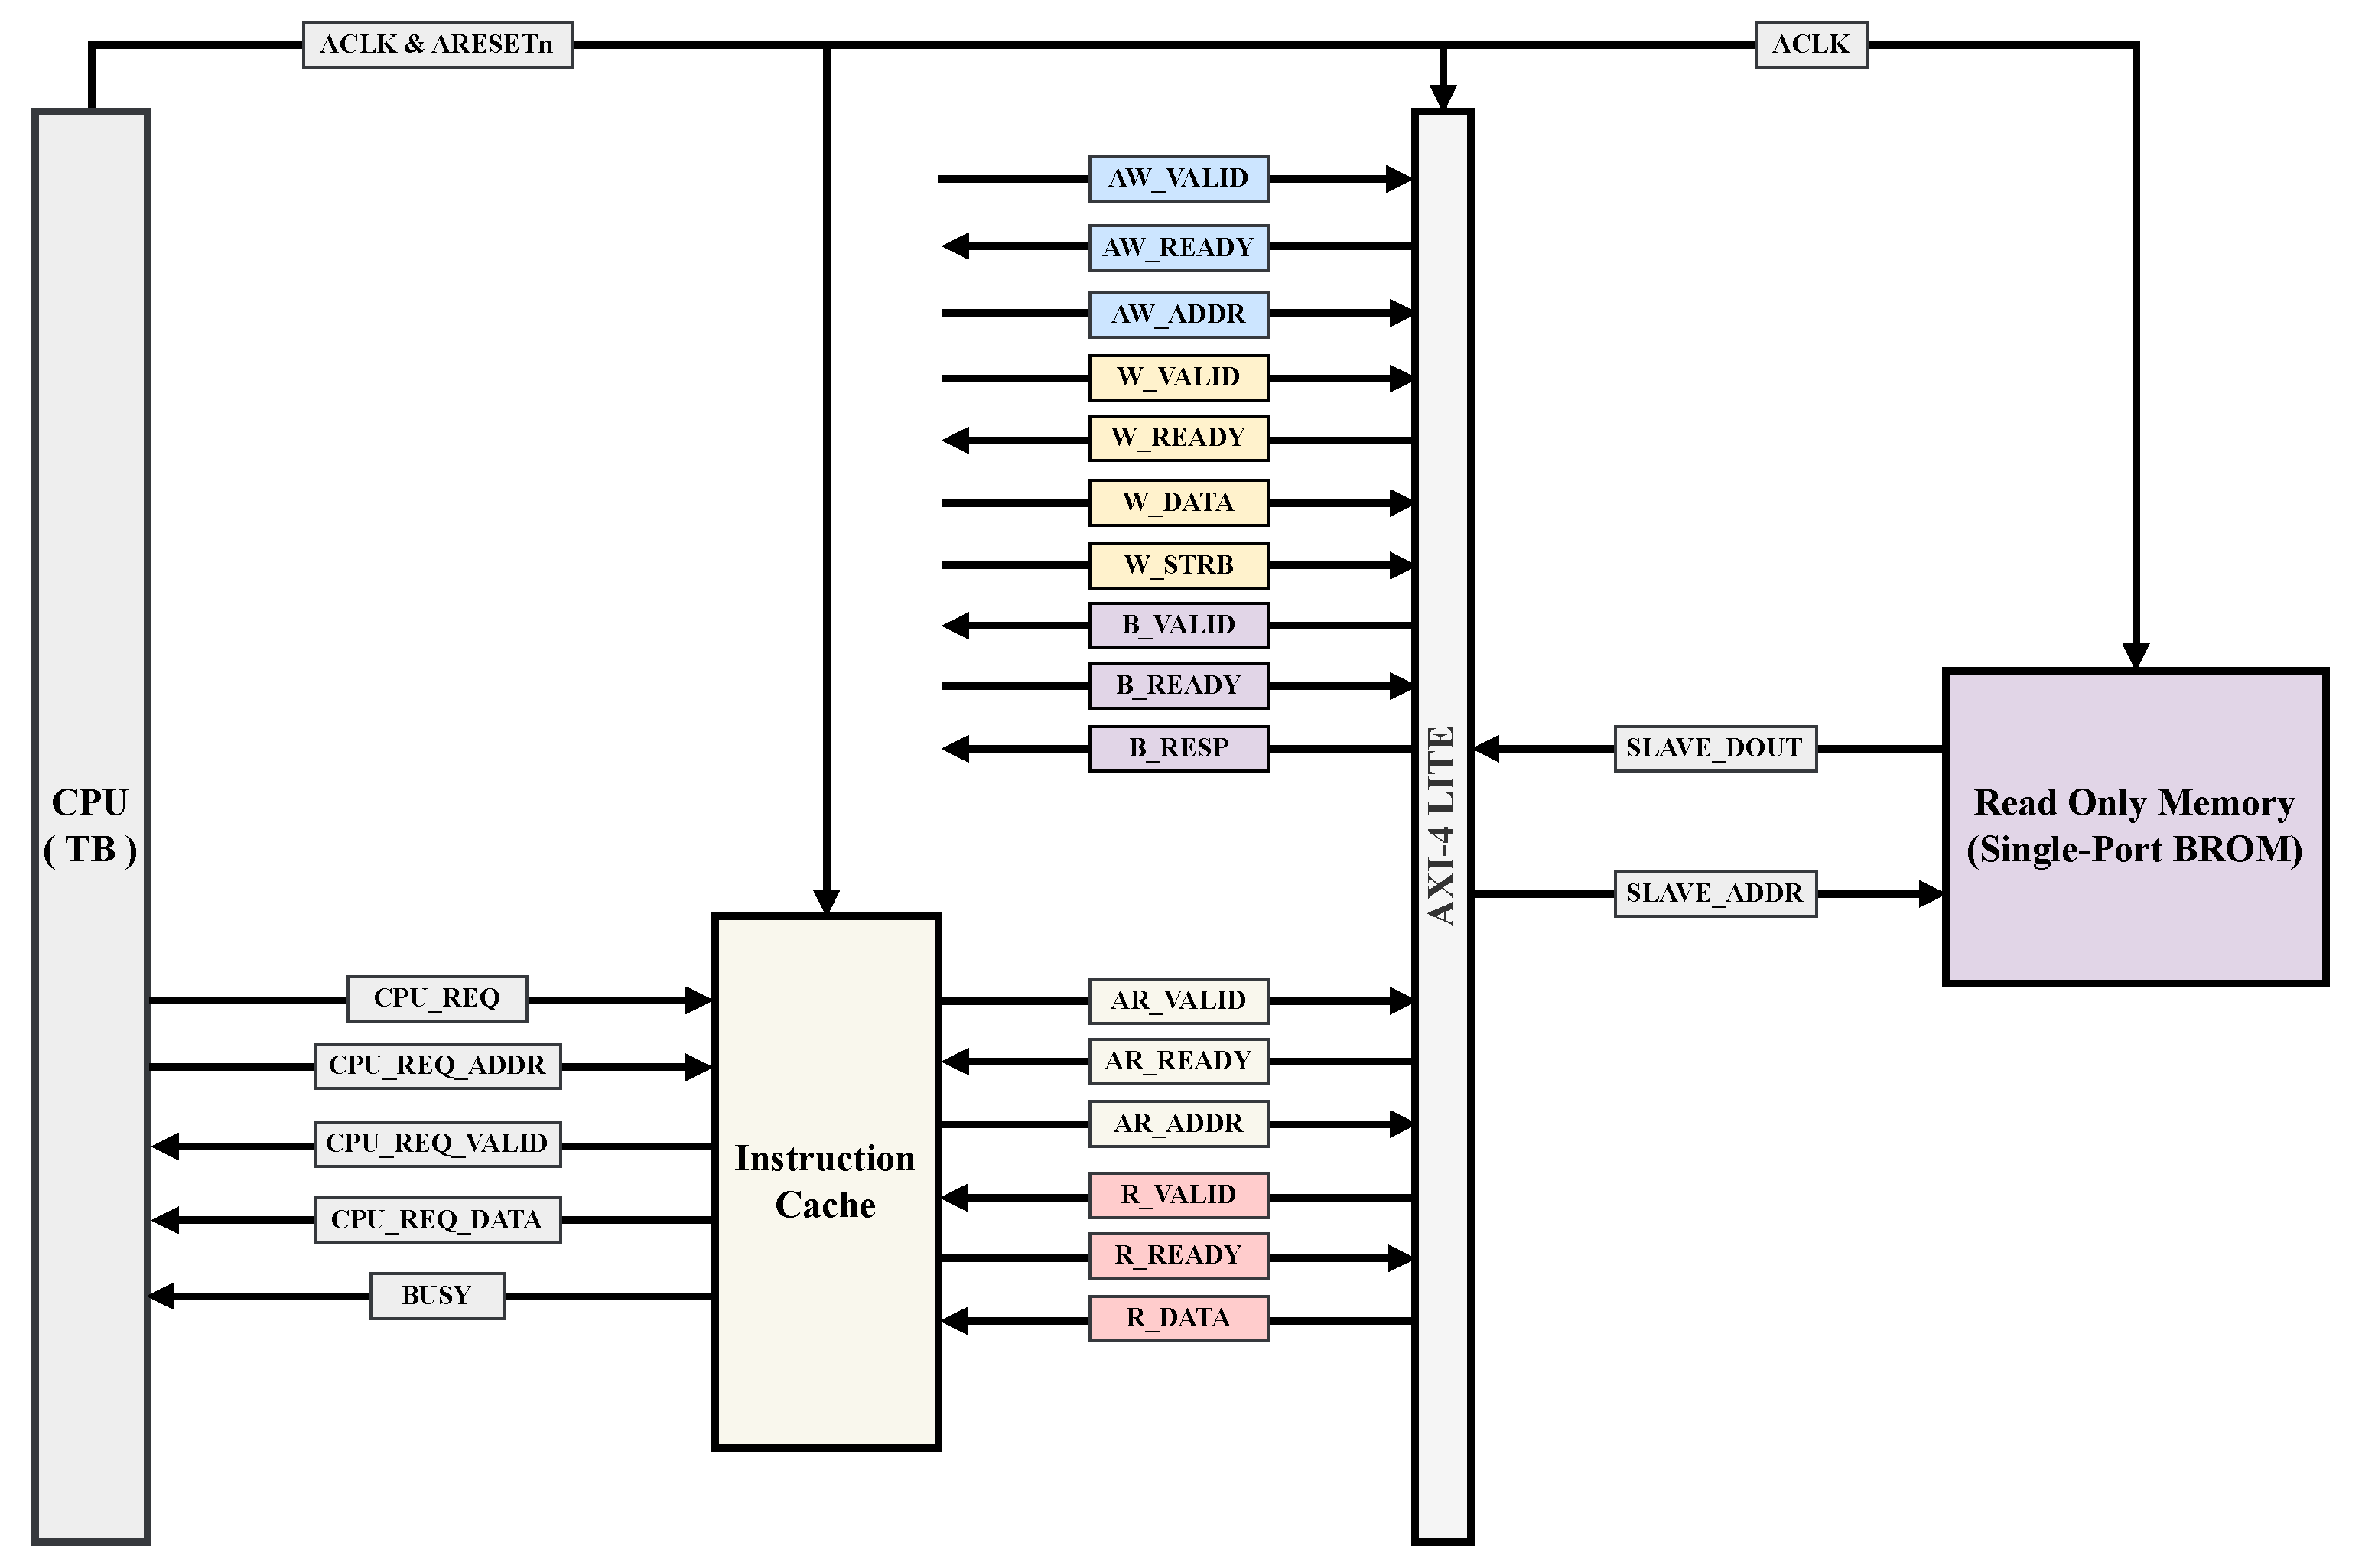
\includegraphics[width=0.9\linewidth]{Cache_AXI_BRAM.pdf}
    \caption{Two-way set-associative Cache with AXI4-Lite to BRAM}
    \label{fig:cache_axi_bram}
\end{figure}

\newpage

\subsection{Data Cache}

In this implementation, the Data Cache employs a Write-Through policy instead of Write-Back with a Write Buffer, which presents an opportunity for future optimization. The Data Cache read operation follows the same logic as the Instruction Cache described in \hyperref[subsec:instruction_cache]{Section~\ref*{subsec:instruction_cache}}. It is important to note that the write and read operations share the same ADDR PORT, and the system follows a Write-First approach similar to Memory. The full RTL design and verification for this module is available \href{https://github.com/akira2963753/Pipelined-RV32-SoC/tree/main/CACHE/D-CACHE}{here}.

\begin{figure}[h]
    \centering
    \includegraphics[width=0.9\linewidth]{DCache_AXI_BRAM.pdf}
    \caption{Data Cache with AXI4-Lite to BRAM}
    \label{fig:d_cache_axi_bram}
\end{figure}

\chapter{RISC-V Processor} 

\newpage
\section{Full System Integration}
In previous chapters, we successfully implemented a 5-stage pipelined RISC-V CPU supporting the RV32I and RV32M instruction sets, an AXI4-Lite Bus Interface with BRAM, an I-Cache (AXI4-Lite to BROM), and a D-Cache (AXI4-Lite to BRAM). In this chapter, we will integrate both caches into the CPU to complete the \textbf{Final RISC-V Processor}, as you can see the Figure 5.1.

It is worth noting that in this chapter, some of the modules introduced in Chapter 3 will be updated with additional control signals or logic to accommodate the cache integration. However, the overall architecture remains largely unchanged.

The integration of the I-Cache is relatively straightforward : while waiting for a valid instruction read (a cache miss or pending fetch), we simply \textbf{disable write-enable for the IF/ID pipeline registers} and \textbf{stall the Program Counter (PC)} to prevent it from updating. This effectively freezes the front-end until the instruction is ready.

Integrating the D-Cache is considerably more complex. Because memory read and write operations spend multiple clock cycles, the entire processor must stall until the transaction completes successfully. To achieve this, \textbf{stall signals must be asserted across all pipeline stages.} 

Furthermore, extra care must be taken to ensure that a \textbf{Branch\_Taken signal is not triggered during a stall}, which prevents illegal state transitions or incorrect instruction execution. We can determine the completion of a write operation by monitoring the AXI-4 Lite response via \textbf{BVALID \&\& BREADY}. For read operations, we track the status through \textbf{CPU\_REQ\_VALID}. Ultimately, whenever the D-Cache is in a \textbf{busy state}, the entire pipeline must remain stalled.

\begin{figure}[h]
    \centering
    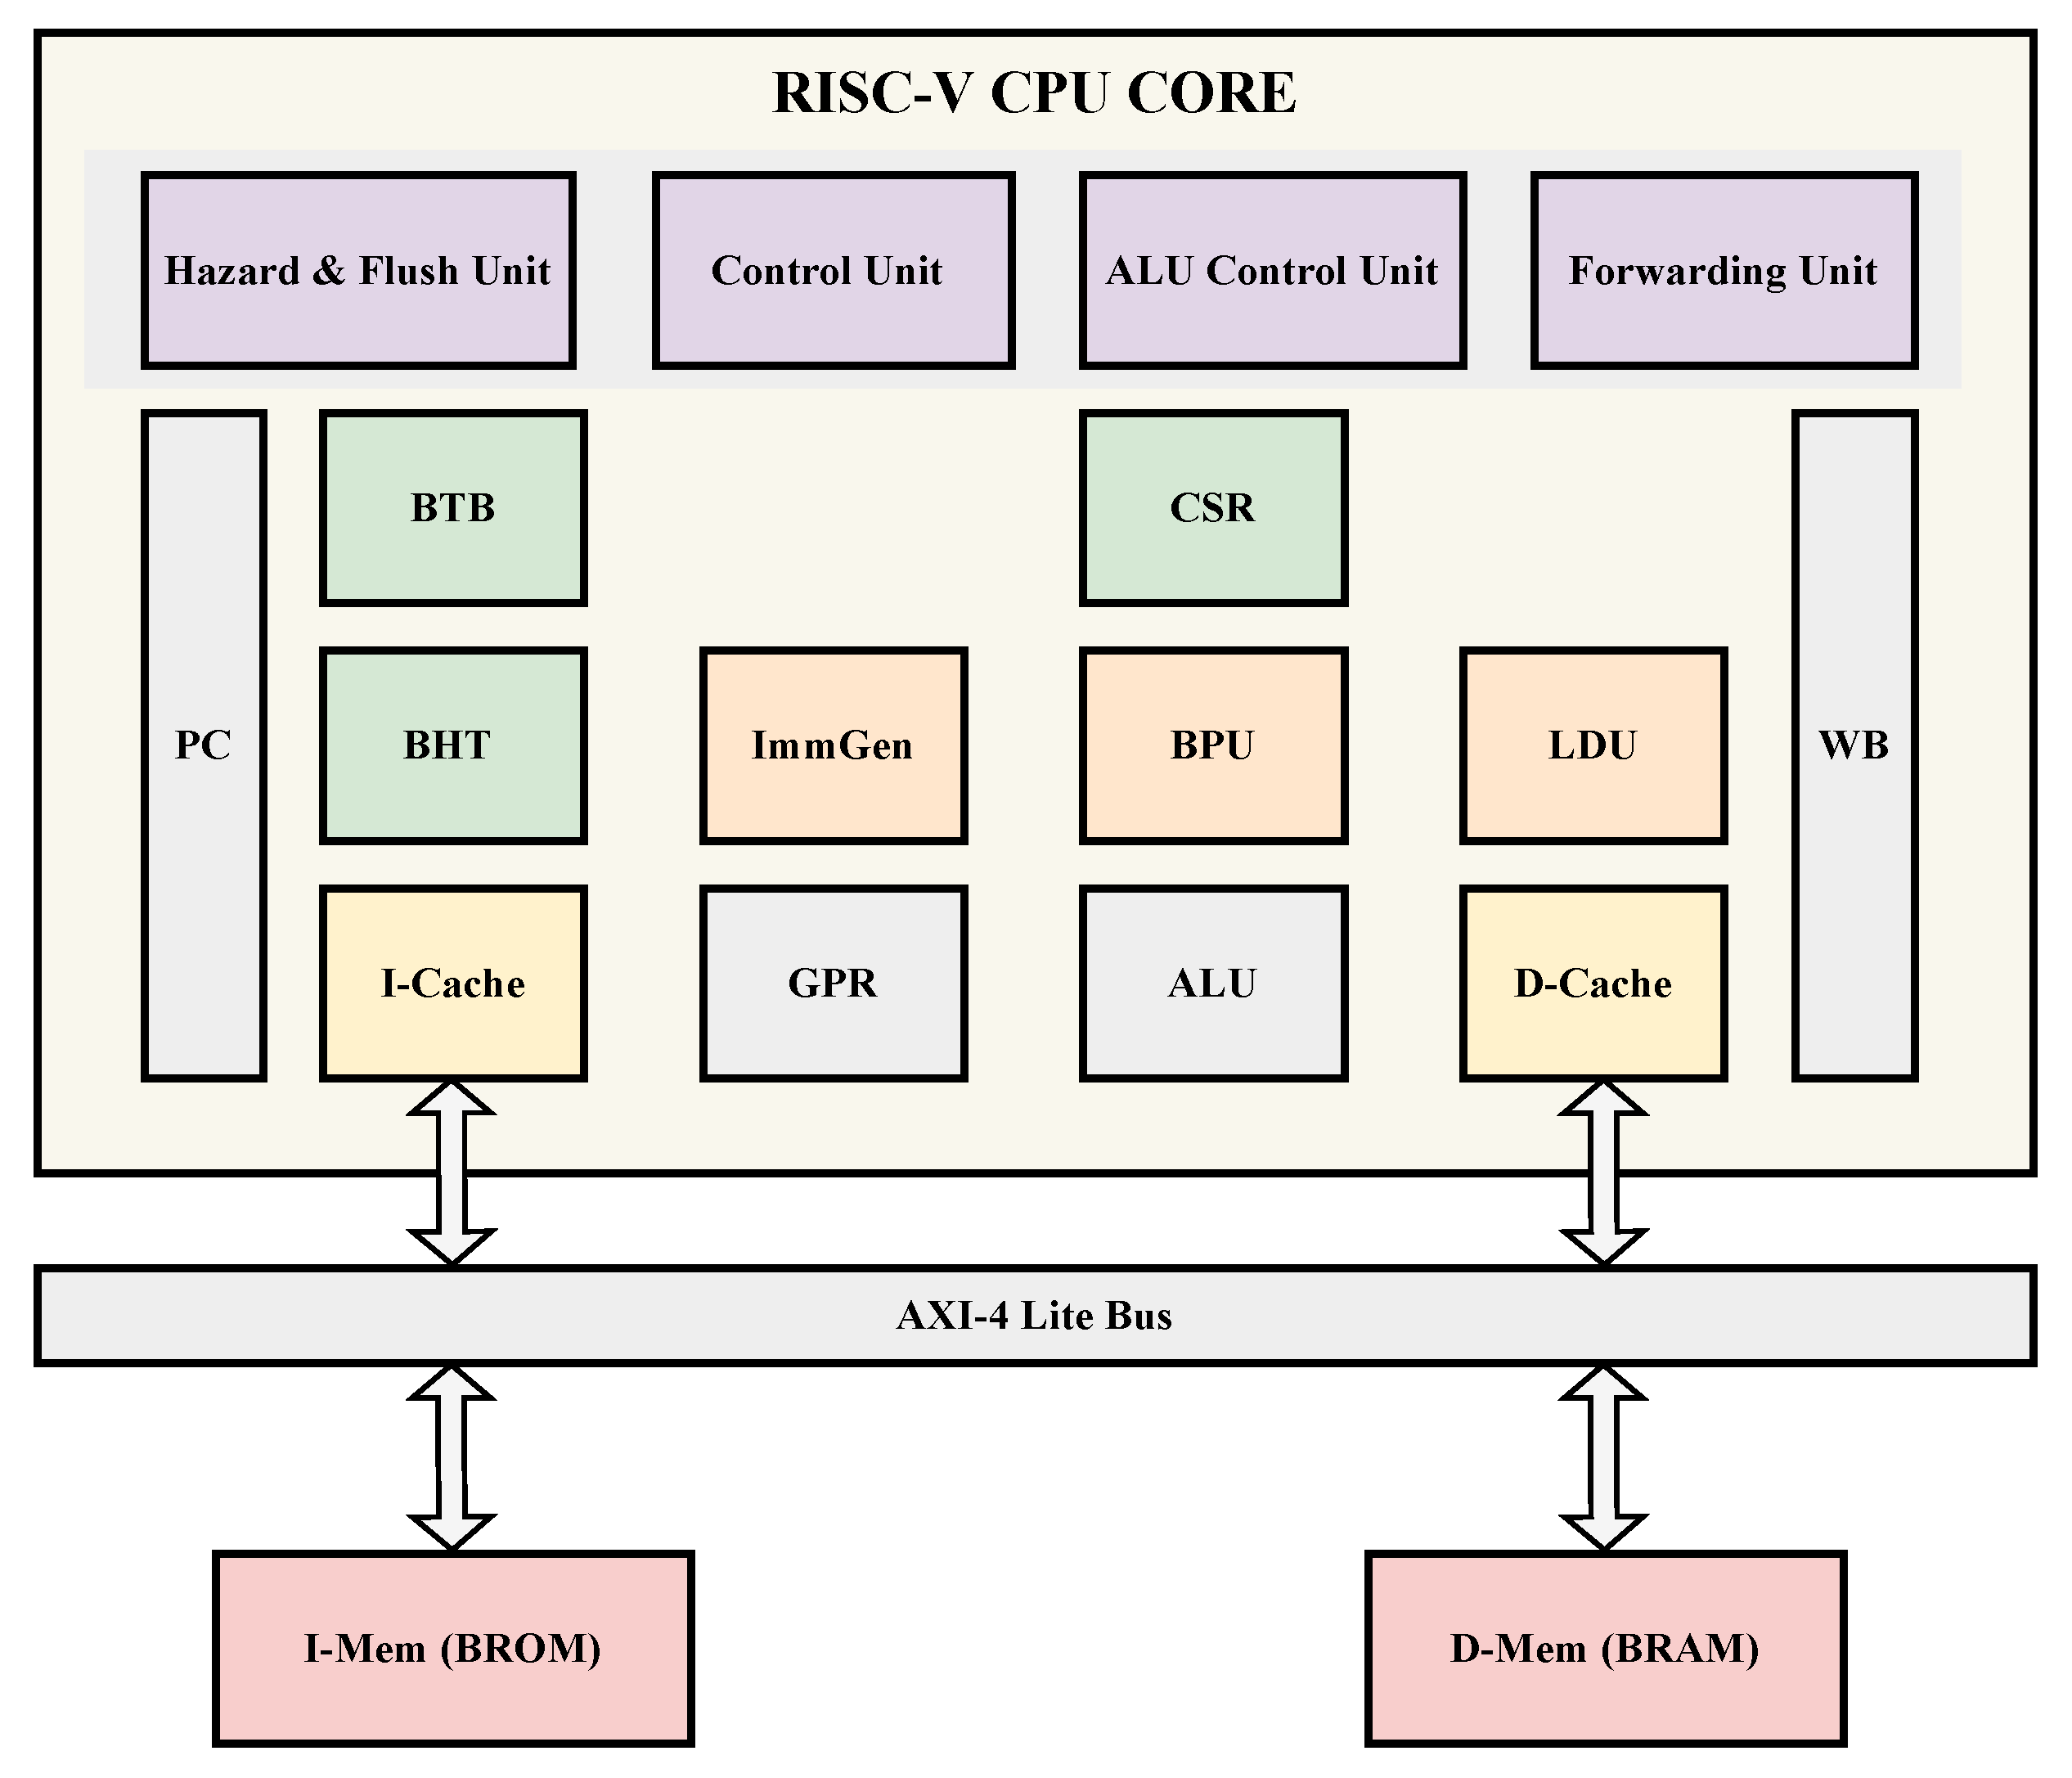
\includegraphics[width=0.7\linewidth]{RISCV_ALL.pdf}
    \caption{RISC-V Processor Overview}
    \label{fig:riscv_all}
\end{figure}

\newpage
\section{System-Level Verification}
The verification process remains consistent with the flow established in Section 3.15, with a few key additions to the automation suite. We have updated \href{https://github.com/akira2963753/Pipelined-RV32-SoC/blob/main/RISC-V%20CPU%20CORE/Verify_Script.py}{Verify\_Script.py} to include a script that converts IM.dat into a .coe format, specifically for the Instruction Memory (BROM IP).

Furthermore, to facilitate the rapid export of Data Memory content via the TestBench, we opted not to use the Vivado-generated BRAM IP. Instead, we implemented a custom module, \href{https://github.com/akira2963753/Pipelined-RV32-SoC/blob/main/RISC-V%20CPU%20CORE/RTL/D_BRAM.v}{D\_BRAM.v}, which replicates the IP's functionality while allowing for easier file I/O operations and data extraction.

More importantly, to accelerate the verification process, I have written the Vivado simulation TCL commands into a \href{https://github.com/akira2963753/Pipelined-RV32-SoC/blob/main/RISC-V-Processor/Script.tcl}{Script.tcl} file and integrated it with the \href{https://github.com/akira2963753/Pipelined-RV32-SoC/blob/main/RISC-V-Processor/Verify_Script.py}{Verify\_Script.py} script to enable automated RTL simulation and verification. Users can choose to run a single Test Case or execute all Test Cases at once.

\begin{figure}[H]
    \centering
    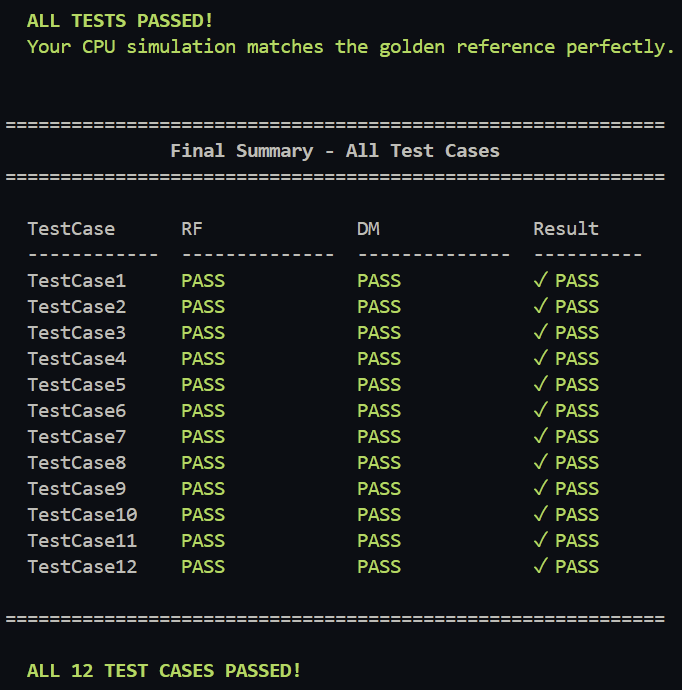
\includegraphics[width=0.65\linewidth]{Result.png}
    \caption{Verification Results}
    \label{fig:result}
\end{figure}

\newpage
\section{Synthesis Results}

The design was synthesised targeting the Xilinx ZCU104 (UltraScale+) platform at a clock frequency of \textbf{250\,MHz}. The table below summarises the key post-synthesis resource utilisation, followed by the complete cell-level breakdown reported by Vivado.

\begin{table}[H]
\centering
\caption{Resource Utilisation Summary}
\begin{tabular}{|l|r|}
\hline
\textbf{Resource} & \textbf{Count} \\
\hline
LUT (total)      & 55{,}911 \\
Flip-Flop (total) & 76{,}491 \\
DSP48E2          & 12       \\
BRAM             & 2        \\
\hline
\textbf{Clock Frequency} & \textbf{250 MHz} \\
\hline
\end{tabular}
\end{table}

\begin{table}[H]
\centering
\small
\caption{Vivado Report Cell Usage}
\begin{tabular}{|l|r|l|r|}
\hline
\textbf{Cell} & \textbf{Count} & \textbf{Cell} & \textbf{Count} \\
\hline
\multicolumn{2}{|l|}{\textit{Clock / Carry}} & \multicolumn{2}{l|}{\textit{LUT}} \\
\hline
BUFG   & 1   & LUT1 & 225    \\
CARRY8 & 717 & LUT2 & 664    \\
\cline{1-2}
\multicolumn{2}{|l|}{\textit{DSP}} & LUT3 & 2{,}677 \\
\cline{1-2}
DSP\_ALU          & 12 & LUT4 & 1{,}646 \\
DSP\_A\_B\_DATA   & 12 & LUT5 & 6{,}316 \\
DSP\_C\_DATA      & 12 & LUT6 & 44{,}383 \\
\cline{3-4}
DSP\_MULTIPLIER   & 12 & \multicolumn{2}{l|}{\textit{MUX}} \\
\cline{3-4}
DSP\_M\_DATA      & 12 & MUXF7 & 18{,}036 \\
DSP\_OUTPUT       & 12 & MUXF8 & 8{,}343  \\
\cline{3-4}
DSP\_PREADD       & 12 & \multicolumn{2}{l|}{\textit{Memory}} \\
\cline{3-4}
DSP\_PREADD\_DATA & 12 & RAMB18E2 & 1 \\
\cline{1-2}
\multicolumn{2}{|l|}{\textit{Flip-Flop}} & RAMB36E2 & 1 \\
\cline{1-2}
FDCE & 10{,}942 & \multicolumn{2}{l|}{\textit{I/O Buffer}} \\
\cline{3-4}
FDPE & 5        & IBUF & 2  \\
FDRE & 65{,}544 & OBUF & 32 \\
\hline
\end{tabular}
\end{table}

\end{document}